%%
%% Copyright 2007-2020 Elsevier Ltd
%%
%% This file is part of the 'Elsarticle Bundle'.
%% ---------------------------------------------
%%
%% It may be distributed under the conditions of the LaTeX Project Public
%% License, either version 1.3 of this license or (at your option) any
%% later version.  The latest version of this license is in
%%    http://www.latex-project.org/lppl.txt
%% and version 1.3 or later is part of all distributions of LaTeX
%% version 1999/12/01 or later.
%%
%% The list of all files belonging to the 'Elsarticle Bundle' is
%% given in the file `manifest.txt'.
%%
%% Template article for Elsevier's document class `elsarticle'
%% with harvard style bibliographic references

\documentclass[preprint,12pt,authoryear]{elsarticle}

%% Use the option review to obtain double line spacing
%% \documentclass[authoryear,preprint,review,12pt]{elsarticle}

%% Use the options 1p,twocolumn; 3p; 3p,twocolumn; 5p; or 5p,twocolumn
%% for a journal layout:
%% \documentclass[final,1p,times,authoryear]{elsarticle}
%% \documentclass[final,1p,times,twocolumn,authoryear]{elsarticle}
%% \documentclass[final,3p,times,authoryear]{elsarticle}
%% \documentclass[final,3p,times,twocolumn,authoryear]{elsarticle}
%% \documentclass[final,5p,times,authoryear]{elsarticle}
%% \documentclass[final,5p,times,twocolumn,authoryear]{elsarticle}

%% For including figures, graphicx.sty has been loaded in
%% elsarticle.cls. If you prefer to use the old commands
%% please give \usepackage{epsfig}

\usepackage{amsfonts}
\usepackage{booktabs}
\usepackage{siunitx}
\usepackage{url}
\usepackage[hidelinks]{hyperref}
\usepackage[T1]{fontenc}		% Seleção de códigos de fonte.
\usepackage[utf8]{inputenc}		% Codificação do documento (conversão automática dos acentos)
\usepackage{lmodern}			% Usa a fonte Latin Modern
% Para utilizar a fonte Times New Roman, inclua uma % no início do comando acima  "\usepackage{lmodern}"
% Abaixo, tire a % antes do comando  \usepackage{times}
%\usepackage{times}		    	% Usa a fonte Times New Roman
% Para usar a fonte , lembre-se de tirar a % do comando %\renewcommand{\ABNTEXchapterfont}{\rmfamily}, localizado mais abaixo, logo após "Outras opções para nota de rodapé no Sistema Numérico"
\usepackage{lastpage}			% Usado pela Ficha catalográfica
\usepackage{indentfirst}		% Indenta o primeiro parágrafo de cada seção.
\usepackage{color}				% Controle das cores
\usepackage{graphicx}			% Inclusão de gráficos
\usepackage{float} 				% Fixa tabelas e figuras no local exato
\usepackage{chemfig,chemmacros} % Para escrever reações químicas
\usepackage{tikz}				% Para escrever reações químicas e outros
\usetikzlibrary{positioning}
\usepackage{microtype} 			% para melhorias de justificação
\usepackage{pdfpages}
\usepackage{makeidx}            % para gerar índice remissivo
\usepackage{hyphenat}          % Pacote para retirar a hifenizacao do texto
\usepackage[absolute]{textpos} % Pacote permite o posicionamento do texto
\usepackage{eso-pic}           % Pacote para incluir imagem de fundo
\usepackage{makebox}           % Pacote para criar caixa de texto
\usepackage{graphicx}
\usepackage{graphbox}
\usepackage{tasks}
\usepackage{amssymb}
\usepackage{amsmath}
\usepackage{amsthm}
\usepackage{fontawesome5}

% TODO List
\usepackage{todonotes}

\usepackage{svg} % ADDED JORGE FOR SVG

\usepackage[ruled]{algorithm2e}

\usepackage{tikz}
\usepackage{aircraftshapes}

\usetikzlibrary{positioning}

\newcommand{\destaq}[1]{\textcolor{BlueViolet}{\textbf{#1}}}
\renewcommand\todo[1]{\colorbox{green}{#1}}

\definecolor{echodrk}{HTML}{0099cc}
\definecolor{olivegreen}{rgb}{0,0.6,0}
\definecolor{camdrk}{RGB}{0,62,114}

\usetikzlibrary{arrows,shapes}

\definecolor{mygreen}{rgb}{0,0.6,0}

\definecolor{mymauve}{rgb}{0.58,0,0.82}

\usetikzlibrary{arrows,shapes, decorations.pathmorphing,backgrounds,positioning}

\pgfdeclarelayer{background}
\pgfsetlayers{background,main}

\tikzstyle{vertex}=[circle,fill=black!25,minimum size=20pt,inner sep=0pt]
\tikzstyle{selected vertex} = [vertex, fill=red!24]
\tikzstyle{select vertex} = [vertex, fill=blue!24]
\tikzstyle{selectx vertex} = [vertex, fill=green!24]
\tikzstyle{edge} = [draw,thick,-]
\tikzstyle{selected edge} = [draw,line width=5pt,-,red!50]

\usepackage{minted}
\usemintedstyle{vs}

\usepackage{enumitem}
\newlist{todolist}{itemize}{2}
\setlist[todolist]{label=$\square$}
\usepackage{pifont}
\newcommand{\cmark}{\ding{51}}%
\newcommand{\xmark}{\ding{55}}%
\newcommand{\done}{\rlap{$\square$}{\raisebox{2pt}{\large\hspace{1pt}\cmark}}%
\hspace{-2.5pt}}
\newcommand{\wontfix}{\rlap{$\square$}{\large\hspace{1pt}\xmark}}

%% MANOEL: CORREÇÕES PARA ADAPTAÇÃO PARA ARTIGO
\let\chapter\section
\let\section\subsection
\let\subsection\subsubsection
\let\cite\citep
\let\citeonline\citealp
\renewcommand{\refname}{\chapter{References}}


\newtheorem{theorem}{Theorem}[section]
\newtheorem{lemma}[theorem]{Lemma}
\newtheorem{property}[theorem]{Property}

\renewcommand\qedsymbol{$\blacksquare$}

\usepackage{lipsum}				% para geração de dummy text
% ---

% pacotes de tabelas
\usepackage{multicol}	% Suporte a mesclagens em colunas
\usepackage{multirow}	% Suporte a mesclagens em linhas
\usepackage{longtable}	% Tabelas com várias páginas
\usepackage{threeparttablex}    % notas no longtable
\usepackage{array}

\usepackage{subfig}


%% The lineno packages adds line numbers. Start line numbering with
%% \begin{linenumbers}, end it with \end{linenumbers}. Or switch it on
%% for the whole article with \linenumbers.
%% \usepackage{lineno}

%% MANOEL: REMOVE PREPRINT NOTE TO THE FRONTPAGE
\makeatletter
\def\ps@pprintTitle{%
  \let\@oddhead\@empty
  \let\@evenhead\@empty
  \def\@oddfoot{\reset@font\hfil\thepage\hfil}
  \let\@evenfoot\@oddfoot
}
\makeatother

% ---
% compila o sumário e índice
\makeindex
% ---



\begin{document}

\begin{frontmatter}

%% Title, authors and addresses

%% use the tnoteref command within \title for footnotes;
%% use the tnotetext command for theassociated footnote;
%% use the fnref command within \author or \affiliation for footnotes;
%% use the fntext command for theassociated footnote;
%% use the corref command within \author for corresponding author footnotes;
%% use the cortext command for theassociated footnote;
%% use the ead command for the email address,
%% and the form \ead[url] for the home page:
%% \title{Title\tnoteref{label1}}
%% \tnotetext[label1]{}
%% \author{Name\corref{cor1}\fnref{label2}}
%% \ead{email address}
%% \ead[url]{home page}
%% \fntext[label2]{}
%% \cortext[cor1]{}
%% \affiliation{organization={},
%%            addressline={},
%%            city={},
%%            postcode={},
%%            state={},
%%            country={}}
%% \fntext[label3]{}

\title{Graph machine learning for flight delay prediction due to
    holding manouver} %% Article title

\affiliation[1]{organization={Instituto Tecnológico de Aeronáutica},
               addressline={Praça Marechal Eduardo Gomes, 50 - Vila das Acácias},
               city={São José dos Campos},
               postcode={12228-900},
               state={São Paulo},
               country={Brazil}}
\affiliation[2]{organization={Universidade de São Paulo (USP)},
               addressline={Instituto de Ciências Matemáticas e de Computação},
               city={São Carlos},
               postcode={13566-590},
               state={São Paulo},
               country={Brazil}}

\author[1]{Manoel Vilela Machado Neto}
\author[1,2]{Jorge Luiz Franco}
\author[1]{Felipe Alves Neto Verri}


% Abstract
\begin{abstract}
%% Text of abstract
This project models the prediction of flight delays due to holding
maneuvers as a graph problem, leveraging advanced Graph Machine
Learning (Graph ML) techniques to capture complex interdependencies in
air traffic networks. Holding maneuvers, while crucial for safety,
cause increased fuel usage, emissions, and passenger dissatisfaction,
making accurate prediction essential for operational
efficiency. Traditional machine learning models, typically using
tabular data, often overlook spatial-temporal relations within air
traffic data. To address this, we model the problem of predicting
holding as edge feature prediction in a directed (multi)graph where we
apply both CatBoost, enriched with graph features capturing network
centrality and connectivity, and Graph Attention Networks (GATs),
which excel in relational data contexts. Our results indicate that
CatBoost outperforms GAT in this imbalanced dataset, effectively
predicting holding events and offering interpretability through
graph-based feature importance. Additionally, a web-based tool,
Airdelay, allows users to simulate real-time delay predictions,
demonstrating the model's potential operational impact. This research
underscores the viability of graph-based approaches for predictive
analysis in aviation, with implications for enhancing fuel efficiency,
reducing delays, and improving passenger experience.


\end{abstract}

%%Graphical abstract
%%\begin{graphicalabstract}
%\includegraphics{grabs}
%\end{graphicalabstract}

%%Research highlights
%\begin{highlights}
%\item Research highlight 1
%\item Research highlight 2
%\end{highlights}

%% Keywords
\begin{keyword}
%% keywords here, in the form: keyword \sep keyword

%% PACS codes here, in the form: \PACS code \sep code

%% MSC codes here, in the form: \MSC code \sep code
%% or \MSC[2008] code \sep code (2000 is the default)
   Graph Neural Networks \sep Graphs \sep Machine Learning \sep Complex Networks

\end{keyword}

\end{frontmatter}
% Seleciona o idioma do documento (conforme pacotes do babel)
% Se o idioma do texto for inglês, inclua uma % antes do
%      comando \selectlanguage{brazil} e
%      retire a % antes do comando abaixo

% Retira espaço extra obsoleto entre as frases.
\frenchspacing

% ---
% ----------------------------------------------------------
% ELEMENTOS TEXTUAIS
% ----------------------------------------------------------
% Os capítulos são inseridos como arquivos externos

% Capítulo 1 - Introdução
% ---
%% USPSC-Introducao.tex

% ----------------------------------------------------------
% Introdução (exemplo de capítulo sem numeração, mas presente no Sumário)
% ----------------------------------------------------------
\chapter[Introduction]{Introduction}
\label{Introdução}

Efficient last-mile delivery logistics is vital for accurate and timely delivery of goods, which influences customer satisfaction and overall business success \cite{boysen2021lastmile}. The use of drones, also called Unmanned Aerial Vehicles (UAVs), in Last-Mile Delivery improves efficiency by overcoming traffic constraints, reducing delivery times, and lowering operational costs.  For this reason, the literature on Delivery Drones increased significantly in the last few years, as analyzed in \citeonline{DUKKANCI2023}.

The literature related to Last-Mile Delivery Drones is highly heterogeneous, encompassing a diverse array of techniques and problem formulations. This diversity spans from studies involving both drones and trucks in delivery scenarios, linear integer modeling for logistic problem-solving, applications of fuzzy logic to address uncertainties, multi-objective optimization to consider multiple criteria simultaneously, to exclusive investigations focusing solely on drones without the presence of other vehicles, including decentralized models.

In \citeonline{FREITAS2023100094} it is studied the Truck-Drone Delivery Problem, which can be addressed as a variation of TSP (Traveling Salesman Problem) for two agents, using a Mixed Integer Programming (MIP) formulation and a heuristic based on a TSP solver and two metaheuristics: General Variable Neighborhood Search (GVNS) and Tabu Search (TS). At the same time, \citeonline{MOSHREFJAVADI2020290} addresses a near problem, but with multiple drones, using Mixed Integer Linear Programming (MILP) and a heuristic based on Adaptive Large Neighborhood Search (ALNS) and Simulated Annealing (SA). A similar MILP modeling was used in \citeonline{drones7070407} and two hybrid genetic algorithms were evaluated.



When addressing multiple criteria simultaneously in collaborative Truck-Drone Delivery, researchers have employed multi-objective optimization techniques.  \citeonline{9580555} consider flexible time windows and diverse objectives, including minimizing the routing costs of drones and trucks and maximizing customer satisfaction. They improved NSGA-II(Non-dominated Sorting Genetic Algorithm) and used a posterior heuristic for Pareto Local Search(PLS).   Complementing this, \citeonline{ZHANG2022108679} introduces a novel multi-objective optimization model for drone delivery, optimizing economic and environmental goals concurrently. The model addresses dynamic drone flight endurance based on loading rates, using an extended NSGA-II algorithm that proves to be effective in generating high-quality solutions, marking advancements in this field.

%Now, article fuzzy, sentiment and energy.

In another branch, works such as \citeonline{farjana2020last} introduce a systematic multi-criterion, multipersonnel decision-making approach called interval-valued inferential fuzzy TOPSIS, handling fuzziness in decision-making and providing quality drone selection decisions. Another study \citeonline{9672856} considers sustainability in optimizing the vehicle routing problem with drones, utilizing sentiment analysis based on Twitter to determine customer sentiments on environmental protection. The net promoter score index calculated from the sentiment analysis is considered as a coefficient in the penalty function added to the base model, aiming to help logistics companies improve the sustainability of the supply chain. Addressing the aspect of energy efficiency in drone-based last mile delivery, another study \citeonline{10049551} focuses on tactical decisions about the selection of shared fulfillment centers used as launch and recovery locations for drones, fleet size plans, and operational drone route decisions. 

%até aqui sem collision

A new perspective in Last Mile Delivery Drones was introduced in \citeonline{Verri}. The study addressed the last-mile delivery problem from a complex system viewpoint, where the collective performance of the drones is investigated. The delivery system incorporates a \textit{tradable permit model} \cite{AKAMATSU2017178}, based on a financial decentralized market-inspired approach, for airspace use, requiring drones to compete for airspace permits in a distributed manner. The simulation evaluates how different parameters, such as arrival rate and airspace dimensions, impact system behavior in terms of cost, time required for drones to acquire flight permits and airspace utilization. Although the simulation employs a simplified model with naïve agents and disregards drone flight dynamics, it captures interesting properties in the agents' collective behavior, demonstrating satisfactory system performance even under high traffic conditions. Simultaneously, \citeonline{lee2022last} contributes a novel combinatorial double auction bi-objective winner determination problem for last-mile drone delivery. 

As we can see, the Last Mile Delivery Drone problem is very hard and complex. In \citeonline{faical}, the authors characterize the problem through a cyber-physical lens, highlighting challenges related to the physical aspects of airspace in the context of drone operations for last-mile delivery. Their analysis delves into considerations such as air traffic management systems, focusing on the evolving landscape of airspace control. This review underscores the need for optimal usage of airspace, then ensuring the need for collision avoidance. However, collision avoidance is a problem that has not been addressed by most of the cited papers until now. \citeonline{Verri} addresses this systematically within the decentralized approach. Indeed, \citeonline{DUKKANCI2023} highlights collision avoidance and air traffic management as a crucial aspect that needs attention in Last-mile delivery drone problems, as much of the literature tends to overlook this when modeling the problem. 


With this problem of collision avoidance and efficient airspace control in mind, the main idea of our work is solve the Last Mile Delivery Drone problem using a MAPF (Multi-Agent Path Finding) approach, thus not ignoring spatial characteristics natural from the airspace. The problem addressed in this work can easily be seen as multi-objective drone path planning for search and rescue \cite{hayat2020multi}, thus the Last Mile Delivery Drone is per se a MAPF.  As stated in \citeonline{lavalle} and proved in \citeonline{Nebel_2020} the MAPF problem is NP-hard. Then our approach is to use elements of prioritized planning \cite{7138650} and conflict-based search \cite{SHARON201540} to face the computational complexity inherited from MAPF while satisfying the constraints of the reduced problem. Although our algorithm does not guarantee global optimum, it always converges in a finite and bounded polynomial time, which is an improvement compared to the previous algorithms described ( MILPs, MOEAs, Metaheuristics).



Centralized control for airspace management, particularly under the Unmanned Aircraft System Traffic Management (UTM) framework developed by the Federal Aviation Administration (FAA) and NASA, exemplifies the necessity of organized, legislative-backed airspace control \cite{nasa}. The UTM facilitates multiple drone operations beyond visual line of sight (BVLOS) by enabling cooperative interaction between drone operators and the FAA, determining and communicating real-time airspace status. While decentralized models, such as those based on blockchain technology \cite{Verri}, offer novel approaches, they introduce complexities in scalability, regulatory compliance, and operational efficiency that can hinder real-time airspace control. The centralized UTM system, supported by regulatory compliance and legislative backing, ensures effective airspace management, safety, and reliability, fostering the integration of UAV deliveries within existing air traffic systems. The FAA's UTM Implementation Plan \cite{9256745} and ongoing evaluations highlight the continual refinement of this centralized approach, emphasizing its critical role in future UAV operations. 


In this study, we propose a novel approach to tackle the Last Mile Delivery Drone problem by employing a Multi-Agent Path Finding (MAPF) strategy. Leveraging elements of prioritized planning and conflict-based search, our algorithm aims to address the computational complexity inherent in the MAPF problem. Unlike previous algorithms such as MILPs and MOEAs, our heuristic guarantees convergence in finite and bounded polynomial time, representing a significant advancement. Our graph-based approach, employing Breadth-First Search (BFS) on temporal grids, enhances the efficiency of our solution. Also, we propose a hybrid method, that combines the heuristic and the MILP. We further present experimental results, comparing our approach with a MILP-based solution and evaluating its performance in the hybrid approach that combines the time found by the heuristic and the MILP solution. Finally, a qualitative comparison between our centralized approach and the decentralized, proposed in \citeonline{Verri}, is presented. The use of a graph-based heuristic offers distinctive advantages, and our experiments shed light on its efficacy in solving the complex Last Mile Delivery Drones problem.

Therefore, in what follows, we describe the main contributions
of this work:
\begin{itemize}
    \item We develop a MILP model to solve the LMDD problem exactly. This model offers a novel method to adapt the MAPF solution to the LMDD context, allowing for drone take-offs, waiting in airspace, and correct landings.
    \item We propose a heuristic algorithm to address the LMDD problem. The primary advantage of our heuristic lies in its graph-based structure, which can be adapted to higher dimensions and weighted sets in the LMDD context. Additionally, our heuristic is polynomially bounded with a low computational cost, representing a novel contribution to the current literature on drone delivery solutions.
\end{itemize}




This monograph is organized as follows. In Section 2 we present the problem definition and the new property. The proposed solution approach is described in Section 3, while the results of the computational experiments are presented in Section 4. Finally, in Section 5 conclusions are drawn.


% ---

% ---
% Capítulo 2

\chapter[Theoretical Framework]{Theoretical Framework and Related Works}
\label{TheoreticalFramework}

Graph machine learning can be tracked backwards to the problem of `learning' on data that is inherently a graph \cite{silva2016machine, JMLR:Perozzi} or can be modeled as a graph \cite{verri2013,grape2020}. This field encompasses a variety of tasks, including node/edge classification, network construction, link prediction, graph classification, graph cut/partitioning, network embeddings, graph coarsening/reduction, which rely on learning representations from graph-structured data. Over the last decades, researchers have developed numerous approaches to tackle these challenges, initially these techniques were most developed by complex networks researchers. However, in the last decade with the advancements in deep learning, the field has seen a significant shift towards the merging of three main communities: graph signal processing, deep learning and complex nets.

As described, defining the field of graph machine learning is not straightforward, as it encompasses a broad range of methods and applications. The tasks mentioned above are just a few examples of the many challenges that can be addressed through graph-based learning techniques. For clarity, these tasks can be categorized into three main learning paradigms: supervised, unsupervised, and semi-supervised learning. In this study, we are interested on the (semi-)supervised learning paradigm, which encompasses a variety of techniques designed to leverage learning to (partially-)labeled data \cite{verri2018advantages,amanciof}. But we can refine even more, in fact, this work will focus in the subset of graph elements prediction(classification/regression) methods.

In this chapter, we provide an overview of the theoretical framework of graph machine learning for node/edge prediction. Here we consider the division of the field into \texttt{classical} graph learning and \texttt{deep} graph learning, where here `classical' refers to the machine learning techniques applied to graphs before the advent of graph neural networks, where standard ML algorithms were applied to graph data and the topological information measures were encoded as features together with the tabular data  \cite{costa2007characterization, silva2016machine}. This bipartition is what will pave the way of our explanation, since the last decade has seen a complex interplay between these two approaches. The field's evolution can be traced back to when \citeonline{bruna2013spectral} introduced one of the first GNN architectures leaned on the theory of graph signal processing. Concurrently, researchers were developing node embedding techniques like DeepWalk \cite{perozzi2014deepwalk} and node2vec \cite{grover2016node2vec}, which bridged classical and deep approaches while remaining using complex networks concepts. The subsequent years saw a surge in GNN architectures, including Graph Convolutional Networks(GCNs) \cite{kipf2016semi} and GraphSAGE \cite{hamilton2017inductive}, marking a shift towards more sophisticated deep learning approaches for graphs and the unification of the field.  

In the following sections, we explain each subset, their theory and applications, and how they have evolved over time. We also discuss the challenges and limitations of these methods.

\section{Classical graph learning}

These early efforts focused on shallow learning techniques such as feature engineering, graph traversal algorithms, and spectral methods, which laid the foundation for understanding graph structure and dynamics. Methods like community detection, centrality measures, and link prediction \cite{silva2016machine} became key tools for analyzing large-scale networks in areas such as social science, biology, and infrastructure systems \cite{newman2018networks,boccaletti2006complex}. A significant focus of these techniques was to develop graph-based features that could be integrated into traditional machine learning models, effectively transforming graph data into a format compatible with standard algorithms like logistic regression, decision trees, and support vector machines. By encoding graph topology through hand-crafted features, such as connectivity and centrality, researchers could leverage these features for tasks like classification, regression, and clustering in tabular machine learning frameworks.

Among these features, centrality measures became particularly important due to their ability to capture the relative importance or influence of nodes in a graph, not just nodes \cite{bonacich1987power}, but other graph elements such as edges \cite{Lu2013edgebetw, brohl2019centrality} and hyperedges \cite{tudisco2021hyperedge}. Centrality measures, such as degree, betweenness, and closeness, served as input features in machine learning pipelines, helping to predict outcomes based on the structural role of nodes within the network. 

Spectral centrality, particularly eigenvector centrality \cite{bonacich1987power}, has proven valuable in machine learning applications due to its ability to identify globally influential nodes. Eigenvector centrality assigns a score to each node by considering not only its direct connections but also the centrality of its neighbors, which results in a recursive definition. Mathematically, the eigenvector centrality $x$ of a node in a graph can be defined as the solution to the equation $Ax = \lambda x$, where $A$ is the adjacency matrix of the graph, and $\lambda$ is the largest eigenvalue, thus $x$ is the eigenvector associated with the largest eigenvalue. This relationship arises from the fact that the centrality of a node is proportional to the sum of the centralities of its neighbors, if we normalize the adjacency we get an stochastic matrix and then $\lambda =1 $ is the largest eigenvalue, named the \texttt{Perron vector}. The eigenvector centrality captures both local and global structure in a network, making it a powerful feature for tasks such as node classification, ranking, and recommendation systems. A related and widely used spectral measure is PageRank \cite{brin1998pagerank}, which extends the idea of eigenvector centrality by introducing a damping factor to model random surfing behavior,
\[
PR(v) = \frac{1 - d}{N} + d \sum_{u \in \mathcal{N}(v)} \frac{PR(u)}{\text{deg}(u)},
\]
where $PR(v)$ is the PageRank score of node $v$, $d$ is the damping factor, and $\mathcal{N}(v)$ represents the neighbors of node $v$. This iterative computation converges to a stationary distribution of scores, which can be interpreted as the probability of landing on a given node after a long random walk, in this sense the \texttt{Perron vector} signifies the convergence of the process in the infinite. PageRank has been widely used in ranking tasks, such as identifying important websites in search engines or recommending influential users in social networks.

However, these spectral-based centralities come with limitations. Eigenvector centrality requires the computation of the principal eigenvector of the adjacency matrix, which involves finding the largest eigenpair problem. This has a time complexity of $\mathcal{O}(n^2 d)$ for exact methods, where $n$ is the number of nodes in the graph and $d$ is the ratio of convergence for the power method. Furthermore, spectral methods can suffer from limitations rooted in the Perron-Frobenius theorem, which guarantees the existence of a unique largest eigenvalue only for irreducible, non-negative matrices. For graphs that are disconnected or have negative weights, these conditions are violated, and the eigenvector centrality may not be well-defined or interpretable. That is, the adjacency matrix should be non-negative and irreducible, where we could use the Perron test $\sum A^k > 0$ to see if the graph is strongly connected.  These centralities also tend to be node-centric, lacking a direct extension to edge importance. For edge centrality, betweenness remains crucial, particularly in directed graphs, where the structural role of links (edges) must be considered to capture flow dynamics. Additionally, spectral centralities can be sensitive to noise and small perturbations in the graph structure, leading to instability in the centrality scores. Despite these challenges, spectral centrality remains a powerful tool for machine learning tasks that benefit from capturing global graph structure, provided that the computational and stability issues can be managed.


\section{Deep graph learning}

The rise of deep learning has revolutionized the field of graph machine learning, enabling the development of more powerful and scalable models for graph data. Graph neural networks can be divide in two main categories: spectral-based and spatial-based. Here is a trick thing, the GCN architecture \cite{kipf2016semi} is commonly divulgated as a spatial-based method, since it is more intuitive talking about the convolution operation in the spatial domain, where we simply aggregate information from the immediate neighbors. However, the GCN is a spectral-based method, in fact, it can be thought as a simplification of the first spectral GNN \cite{bruna2013spectral} proposed and that builds the math behind GCNs. That said, first we introduce the spectral-based GNNs and then the spatial-based ones.

\subsection{Spectral-based GNNs}

Spectral methods are rooted in graph signal processing. The core idea is that a signal on a graph can be represented as node features, where each feature vector at a node corresponds to a `signal' defined over the graph. In this context, the graph Laplacian $\mathcal{L} = D - A$, where $D$ is the degree matrix and $A$ is the adjacency matrix, plays a crucial role. It captures the structure of the graph and can be used to perform operations analogous to Fourier transforms in classical signal processing. Spectral methods can be categorized into two types: eigenvalue-based, where the focus is on creating a graph filter in the Fourier domain, and eigenvector-based, where the goal is to use a spectral basis to decompose the signal \cite{bo2023surveyspectralgraphneural}.

\citeonline{bruna2013spectral} introduced the first spectral Graph Neural Network (GNN), termed the Spectral CNN (SCNN), which aimed to translate ideas from standard Convolutional Neural Networks for images to graphs. The SCNN leverages the spectral decomposition of the graph Laplacian $\mathcal{L} = U \Lambda U^T$ to define a filter convolution operation in the Fourier domain. In this framework, the graph Fourier transform of a signal $f$ is represented as $\hat{f} = U^T f$, and the convolution operation ($\star$) is defined as $g_{\theta} \star f = U g_{\theta} U^T f$, where $g_{\theta}$ is a learnable filter parameterized by $\theta$. While powerful, the SCNN faces significant challenges: it requires $\mathcal{O}(n^3)$ computational complexity to calculate the entire graph spectrum, which is prohibitively expensive for large graphs. Moreover, the non-localized nature of eigenvectors means global information can overshadow local structural details, leading suboptimal balance between local and global information aligned with a huge parameter complexity \cite{usgnn}.

To address these limitations, ChebNet\citeonline{defferrard2016convolutional} introduces Chebyshev polynomials to approximate spectral filters, effectively reducing computational complexity while preserving the ability to capture localized patterns in the graph structure. The main ideia is to redefine our previous filtering operation to $ g_{\theta}(\mathcal{L} ) f = \sum_{k=0}^{K-1} \theta_k T_k(\widetilde{\mathcal{L}}) f $, where $T_k(\widetilde{\mathcal{L}}) = $ is the Chebyshev polinomial of order k evaluated at the scaled Laplacian $\widetilde{\mathcal{L}} = 2 \frac{\mathcal{L}}{\lambda_\text{max}} - I_n$. This innovation not only makes spectral GNNs more scalable to larger graphs, since we just need to calculate the first eigenpair ($\mathcal{O}(n^2)$ through the power method) for the approximations, but also enhances their ability to balance local and global information processing. In fact, the filters are $K$-localized for polinomials of order $K$, that is intuitive by remembering that $\mathcal{L} ^K$ represents the paths with length less or equal to $K$.  
The ChebNet laid the foundation for GCNs \cite{kipf2016semi}. Although GCNs are commonly referred to as spatial methods, their underlying principle is rooted in the truncation of the Chebyshev expansion to $K=1$, which limits the filter to first-order neighbors. This simplification reduces computational complexity significantly while preserving effectiveness. Instead of requiring the full spectral decomposition of the Laplacian matrix, GCNs use a localized approximation of the graph convolution, expressed as: $g_{\theta} \star f \approx \theta (I_n + \widetilde{A}) f$, where $\widetilde{A} = D^{-\frac{1}{2}} A D^{-\frac{1}{2}}$ is the normalized adjacency matrix, where $A$ is the adjacency matrix, and $D$ is the degree matrix. This approximation results in an efficient propagation rule that aggregates information from a node's immediate neighbors while updating the node's features. This propagation mechanism is often confused as a spatial method because it effectively propagates information from adjacent nodes—akin to a spatial neighborhood aggregation. Although its already a simple model, results have shown that GCNs can achieve state-of-the-art performance on a variety of tasks with even more simplifications \cite{wu2019simplifying}.

However, as we can note, all these spectral methods works just in undirected graphs, since it needs the spectral decomposition


\subsection{Spatial-based GNNs}

Spatial-based GNNs differ from spectral-based approaches by directly leveraging the graph structure to perform convolutions in the spatial domain, rather than relying on the spectral decomposition of graph operators like the Laplacian. In spatial-based methods, the convolution operation is interpreted as an aggregation of node features from a node's local neighborhood, akin to how standard convolutional neural networks aggregate pixel information from nearby regions in image data. These methods operate by iteratively updating node representations by propagating information between neighboring nodes, making them intuitive and highly scalable for large-scale graphs.

The general framework for message passing in spatial-based GNNs can be described as follows. For each node $i$, at layer $t$, we aggregate the features of its neighbors $\mathcal{N}(i)$ to produce an updated node embedding: $\mathbf{m}_i^{(t+1)} = \text{AGGREGATE}^{(t)} \left( \left\{ \mathbf{h}_j^{(t)} : j \in \mathcal{N}(i) \right\} \right)$, where $\mathbf{h}_j^{(t)}$ is the feature of neighboring node $j$ at layer $t$. Then, we update the node $i$'s representation: $\mathbf{h}_i^{(t+1)} = \text{UPDATE}^{(t)} \left( \mathbf{h}_i^{(t)}, \mathbf{m}_i^{(t+1)} \right)$, where $\text{AGGREGATE}^{(t)}$ is a neighborhood aggregation function, and $\text{UPDATE}^{(t)}$ is the node update function.

The general idea behind spatial-based GNNs is that, for each node, we aggregate the features of its neighbors to produce an updated node embedding. A key example of this is the GraphSAGE architecture \cite{hamilton2017inductive}, which computes node representations by sampling and aggregating features from the node's neighbors. The GraphSAGE model employs several types of aggregation functions, including mean, LSTM-based, and pooling aggregators, which allow for flexible and inductive learning on large graphs. In particular, GraphSAGE enables the generation of embeddings for unseen nodes, making it suitable for inductive learning tasks, where the model needs to generalize to new nodes that were not present during training. Unlike spectral-based methods, which are constrained to a fixed graph size and structure due to their reliance on the graph Laplacian, spatial-based GNNs are inherently more flexible and can be applied to dynamic and evolving graphs. These models perform neighborhood aggregation locally, and therefore do not require the global knowledge of the graph structure that spectral methods need. This flexibility makes them particularly useful for large-scale graphs and for graphs where the structure may change over time, such as social networks or knowledge graphs.


Another prominent spatial-based GNN is the Graph Attention Network (GAT) \cite{velickovic2017graph}, which introduced attention mechanisms into graph learning. GAT models learn to assign different weights to the neighbors of a node, allowing the model to focus more on the most relevant neighbors during the feature aggregation process. This is achieved using a self-attention mechanism, where the importance of neighboring nodes is learned through a shared attention coefficient, $
e_{ij} = \text{LeakyReLU}(\mathbf{a}^T [\mathbf{W} \mathbf{h}_i || \mathbf{W} \mathbf{h}_j]) $, where $e_{ij}$ represents the attention coefficient between nodes $i$ and $j$, $\mathbf{W}$ is a learnable weight matrix, $\mathbf{h}_i$ and $\mathbf{h}_j$ are the feature vectors of nodes $i$ and $j$, and $||$ denotes concatenation. The attention coefficients are then normalized across all of a node's neighbors using the softmax function, $
\alpha_{ij} = \frac{\exp(e_{ij})}{\sum_{k \in \mathcal{N}(i)} \exp(e_{ik})}
$, this normalization ensures that the attention coefficients sum to 1, allowing the model to perform a weighted aggregation of the neighbors' features, $
\mathbf{h}_i' = \sigma \left( \sum_{j \in \mathcal{N}(i)} \alpha_{ij} \mathbf{W} \mathbf{h}_j \right)$,
here $\mathbf{h}_i'$ is the updated representation of node $i$, and $\sigma$ is a non-linear activation function. By learning attention coefficients, GATs can capture both the importance and the structure of the graph, making them particularly effective in tasks where the relationships between nodes are not equally important, such as in citation networks or social media graphs.

% ---

%\include{6_mathematical_model}

%\include{7_heuristic}



%\include{5_materialsAndMethods}

% ---
% Capítulo 3
% ---
\chapter[Materials and Methods]{Materials and Methods}
\label{Materials}

This chapter details the materials and methods used in our study. Specifically, we will cover the dataset, the model based on CatBoost using graph-derived features, and our approach using Graph Attention Networks (GATs) for predictive modeling. Our dataset includes a range of meteorological, geographical, and flight variables. 

Our objective is to detail and model how to predict if a given aircraft is going to delay due to holding maneuver in a supervised learning setting.

\section{Datasets}
\label{Datasets}

The study utilizes two distinct datasets, each containing 42,336 observations, with identical meteorological, geographical, and flight-related features. These datasets were constructed from a combination of METAR and METAF weather reports, airport and flight specifications sourced from ICEA. Each dataset serves a different predictive modeling purpose—binary classification and regression—and includes tailored labels to reflect these objectives

One of the primary challenges in the classification dataset is its class imbalance, which could impact model performance. Common approaches to address imbalance, such as oversampling or undersampling, have been shown to introduce limitations like overfitting and poor generalization (\cite{zhao2021graphsmote}, Graph SMOTE). For graph machine learning tasks, oversampling is generally problematic due to the risk of introducing artificial connectivity patterns, while undersampling can lead to loss of critical structural information. Therefore, we opted to explore model-based techniques without applying these rebalancing methods.

\subsection{Binary Classification Dataset}
The binary classification dataset is used to predict the likelihood of a holding maneuver occurring for a given flight. In this dataset, the label is a binary value:
\begin{itemize}
    \item \textbf{Class 0 (No Holding)}: Represents flights with no holding delays, comprising 41,616 samples.
    \item \textbf{Class 1 (Holding)}: Indicates flights with holding delays, comprising only 720 samples.
\end{itemize}
This significant imbalance between the classes adds complexity to the classification task, as the model needs to accurately predict a rare event within the data.

\subsection{Regression Dataset}
The regression dataset aims to predict the exact duration of holding delays in seconds, thus providing a continuous label for each observation:
\begin{itemize}
    \item \textbf{Holding Time (Seconds)}: For this dataset, each holding event is represented by a floating-point number indicating the holding time in seconds. This approach enables a finer-grained analysis and can potentially improve operational insights by quantifying delay duration rather than merely classifying its occurrence.
\end{itemize}


\subsection{Meteorological Features}
The dataset includes a comprehensive range of meteorological variables from both METAR and METAF reports:

\begin{itemize}
    \item \textbf{Wind Direction:} \texttt{metar\_wind\_direction}, \texttt{metaf\_wind\_direction}
    \item \textbf{Wind Speed:} \texttt{metar\_wind\_speed}, \texttt{metaf\_wind\_speed}
    \item \textbf{Wind Gusts:} \texttt{metar\_wind\_gust}, \texttt{metaf\_wind\_gust}
    \item \textbf{Visibility:} \texttt{metar\_visibility}, \texttt{metaf\_visibility}
    \item \textbf{Cloud Coverage:} \texttt{metar\_cloudcover}, \texttt{metaf\_cloudcover}
    \item \textbf{Temperature:} \texttt{metar\_temperature}, \texttt{metaf\_temperature}
    \item \textbf{Dew Point:} \texttt{metar\_dewpoint}, \texttt{metaf\_dewpoint}
    \item \textbf{Altitude:} \texttt{metar\_elevation}, \texttt{metaf\_elevation}
    \item \textbf{Sky Levels:} \texttt{metar\_skylev1}, \texttt{metar\_skylev2}, \texttt{metar\_skylev3}, \texttt{metar\_skylev4}, \texttt{metaf\_skylev1}, \texttt{metaf\_skylev2}, \texttt{metaf\_skylev3}, \texttt{metaf\_skylev4}
    \item \textbf{Altimeter Setting:} \texttt{metar\_altimeter}, \texttt{metaf\_altimeter}
    \item \textbf{Weather Symbols:} \texttt{metar\_current\_wx1\_symbol}, \texttt{metar\_current\_wx2\_symbol}, \texttt{metar\_current\_wx3\_symbol}, \texttt{metaf\_current\_wx1\_symbol}, \texttt{metaf\_current\_wx2\_symbol}, \texttt{metaf\_current\_wx3\_symbol}
\end{itemize}

\subsection{Geographical Features}
The geographical features include variables based on flight paths and airport information:

\begin{itemize}
    \item \textbf{Flight Distance:} Calculated as the geodesic distance between departure and arrival airports.
    \item \textbf{Airport Altitude:} \texttt{departure\_altitude} and \texttt{arrival\_altitude}, reflecting the elevation of the airports.
    \item \textbf{Latitude and Longitude:} \texttt{departure\_latitude}, \texttt{departure\_longitude}, \texttt{arrival\_latitude}, and \texttt{arrival\_longitude} for geolocation-based analysis.
\end{itemize}

\subsection{Flight-Specific Features}
These features capture specific characteristics related to the flight and any runway head changes:

\begin{itemize}
    \item \textbf{Previous Runway Head Change:} \texttt{prev\_troca\_cabeceira}
    \item \textbf{Runway Head Change in Previous Hour:} \texttt{troca\_cabeceira\_hora\_anterior}
    \item \textbf{Flight Hour:} \texttt{hora\_do\_voo}
\end{itemize}

\section{CatBoost with Graph Features}
\label{sec:catboost_model}

This study employs the CatBoost model, a high-performance gradient boosting library, chosen specifically for its ability to handle categorical features and class imbalance effectively, as well as for its robust handling of noisy data \cite{prokhorenkova2018catboost}. CatBoost has been widely recognized for its superior performance in structured data problems, particularly when compared to other boosting algorithms like XGBoost and LightGBM, thanks to its unique techniques such as ordered boosting and categorical feature encoding. These innovations help prevent overfitting and enhance generalization in class unbalanced problems.

Here, we describe how CatBoost is combined the graph-based features that are extracted of our modeled airports network. These features are derived from the weighted directed graph and enconded as tabular features that are used as input to the model as we describe in the following sections.


\subsection{Graph Representation of the Flight Network}

\begin{figure}[ht]
    \centering
    \begin{tikzpicture}[
        ->, % directed edges
        >=stealth, % arrow tip
        node distance=3cm, % distance between nodes
        airport/.style={circle, draw, minimum size=2cm, font=\Large}, % style for airports
        flight/.style={font=\small} % style for flights
    ]

    % Nodes (Airports)
    \node[airport] (A) {SP \\ \faPlaneDeparture}; % São Paulo with departure icon
    \node[airport] (B) [right of=A] {RJ \\ \faPlaneDeparture}; % Rio de Janeiro with departure icon
    \node[airport] (C) [below of=A] {MG \\ \faPlaneDeparture}; % Minas Gerais with departure icon

    % Edges (Flights)
    \draw[->] (A) to node[flight, above] {\tikz[baseline]{\node[rotate=0]{\faPlane};}} (B); % Flight from SP to RJ, plane icon aligned (0 degrees)
    \draw[->] (B) to node[flight, right] {\tikz[baseline]{\node[rotate=220]{\faPlane};}} (C); % Flight from RJ to MG, plane icon rotated 270 degrees
    \draw[->] (C) to node[flight, left] {\tikz[baseline]{\node[rotate=96]{\faPlane};}} (A); % Flight from MG to SP, plane icon rotated 135 degrees

    \end{tikzpicture}
    \caption{Airports and Directed Flights}
    \label{fig:flight_network_graph}
\end{figure}


To model the interactions in flight data, we represented the problem as a directed graph, depicted in Figure~\ref{fig:flight_network_graph}, where each node represents an airport, here we represent the airports as states of Brazil: SP (São Paulo), MG (Minas Gerais), RJ (Rio de Janeiro). In this network:
\begin{itemize}
    \item Nodes represent airports.
    \item Directed edges represent flights, with each edge directed from the departure airport to the destination airport.
\end{itemize}
Given the frequent occurrence of multiple flights between the same pairs of airports (i.e., multiedges), we have in fact a multigraph, however we abstract it into a weighted directed graph as shown in \ref{fig:multigraph_to_weighted_graph}. Here, each edge's weight corresponds to the total number of flights between a specific pair of airports, transforming multiple directed edges into a single weighted edge. This abstraction allows us to calculate key network metrics more easily, which we then used as features in the CatBoost model.

\begin{figure}[h]
    \centering
    \begin{tikzpicture}[
        ->, % directed edges
        >=stealth, % arrow tip style
        node distance=4cm, % distance between nodes
        airport/.style={circle, draw, minimum size=2cm, font=\Large}, % style for airports
        flight/.style={font=\small, scale=0.8} % smaller size for flights
    ]
    
    % Multigraph (Left Side)
    \node[airport] (A1) {SP \\ \faPlaneDeparture}; % São Paulo with departure icon
    \node[airport] (B1) [right of=A1] {RJ \\ \faPlaneDeparture}; % Rio de Janeiro with departure icon
    \node[airport] (C1) [below of=A1, yshift=-1cm] {MG \\ \faPlaneDeparture}; % Minas Gerais with departure icon
    
    % Multiple flights in the multigraph (non-intersecting paths)
    \draw[->] (A1) to[bend left=20] node[flight, near start] {\tikz[baseline]{\node[rotate=0, scale=0.7]{\faPlane};}} (B1); % Flight 1 from SP to RJ
    \draw[->] (A1) to[bend left=40] node[flight, near start] {\tikz[baseline]{\node[rotate=0, scale=0.7]{\faPlane};}} (B1); % Flight 2 from SP to RJ
    \draw[->] (A1) to[bend left=60] node[flight, near start] {\tikz[baseline]{\node[rotate=0, scale=0.7]{\faPlane};}} (B1); % Flight 3 from SP to RJ
    
    \draw[->] (B1) to[bend right=20] node[flight, near start] {\tikz[baseline]{\node[rotate=270, scale=0.7]{\faPlane};}} (C1); % Flight 1 from RJ to MG
    \draw[->] (B1) to[bend right=40] node[flight, near start] {\tikz[baseline]{\node[rotate=270, scale=0.7]{\faPlane};}} (C1); % Flight 2 from RJ to MG
    
    \draw[->] (C1) to[bend right=20] node[flight, near start] {\tikz[baseline]{\node[rotate=135, scale=0.7]{\faPlane};}} (A1); % Flight 1 from MG to SP
    \draw[->] (C1) to[bend right=40] node[flight, near start] {\tikz[baseline]{\node[rotate=135, scale=0.7]{\faPlane};}} (A1); % Flight 2 from MG to SP
    \draw[->] (C1) to[bend right=60] node[flight, near start] {\tikz[baseline]{\node[rotate=135, scale=0.7]{\faPlane};}} (A1); % Flight 3 from MG to SP
    
    % Transformation arrow
    \node at ($(A1)!0.5!(B1)+(3.5,-2)$) {\Huge $\Rightarrow$};
    
    % Weighted Graph (Right Side)
    \node[airport] (A2) [right=6cm of A1] {SP \\ \faPlaneDeparture}; % São Paulo airport (weighted graph)
    \node[airport] (B2) [right of=A2] {RJ \\ \faPlaneDeparture}; % Rio de Janeiro airport (weighted graph)
    \node[airport] (C2) [below of=A2, yshift=-1cm] {MG \\ \faPlaneDeparture}; % Minas Gerais airport (weighted graph)
    
    % Weighted edges (single paths)
    \draw[->] (A2) to[bend left=20] node[flight, near end, yshift=0.3cm] { $W = 3$ \;} (B2); % Weighted edge from SP to RJ
    \draw[->] (B2) to[bend right=20] node[flight, near end, xshift=0.2cm] {\; \;\;\;\;\; \; $W = 2$  } (C2); % Weighted edge from RJ to MG
    \draw[->] (C2) to[bend right=20] node[flight, near end, xshift=-0.8cm] {  $W=3$  } (A2); % Weighted edge from MG to SP
    
    \end{tikzpicture}
    \caption{Transformation of a multigraph of flights into a weighted directed graph. The multigraph (left) represents multiple flights between airports. In the weighted graph (right), edges are aggregated to show total flights as weights.}
    \label{fig:multigraph_to_weighted_graph}
\end{figure}





\subsection{Graph-based Features}
The graph-based features encode essential structural information about the flight network, capturing connectivity, centrality, and robustness. These features are crucial for understanding the influence of each airport within the network and its potential impact on flight holding patterns. 

Although we have already made this simplification of the multigraph, transforming it into a weighted directed graph, we still need to extract the features from the graph and encode them as tabular data. However, this is not straightforward, as the graph measures are not directly compatible with the model.  

The modelling will impact dramatically in the resulting graph-based features. For instance, we need to calculate edge measures, but this is not so explored as node measures, so the lack of possibilities is a challenge to be overcome.  Another challenge is the direction, that is, we have to create edge measures in a directed weighted graph, which is hard, as we detailed in section \ref{classical_learning}, because most of the complex networks measures proposed are `node centric' and for undirected graphs.

With this in mind, we can observe why the weighted graph transformation was so important, since the measures available for our setting are strongly dependent to the weight (as we will detail later), and our graph is almost totally connected, so in undirected unweighted setting they would be approximately equal, leaving no information. The following graph metrics were calculated from the weighted directed graph:

\begin{itemize}
    \item \textbf{Betweenness Centrality:} Captures the relative importance of each airport in terms of the routes it controls within the network. Higher values indicate airports that serve as critical transit points.
    \item \textbf{Flow Betweenness:} Highlights the flow dynamics of connections, showing how flights tend to route through certain airports, which may correlate with congestion.
    \item \textbf{Edge Connectivity:} Indicates the robustness of airport connections, with higher values signifying more resilient routes between airports that could better handle rerouting needs.
    \item \textbf{Degree Difference:} Measures the disparity between in-degrees and out-degrees at each node, helping to identify key hubs or spokes in the network.
    \item \textbf{Google Matrix:} Based on PageRank centrality, the Google matrix provides a probabilistic transition representation for each airport, which reflects both local and global connectivity.
\end{itemize}

As we can see, these features are not commonly used in the literature. Here is where the weighted network plays a crucial role, edge betweeness centrality \cite{newman2004finding} is constructed using shortest paths in the network, thus the weight will be crucial part of it, since without it the graph is almost fully connected, the shortest path will be almost the same for all pairs of nodes. The same happens with flow betweeness centrality \cite{freeman1991centrality}, that is a measure based on electrial circuits Kirchoff law, more specifically, instead of working with shortest paths, it use the maximum flow that pass through each edge and the weight visualized as capacity will be crucial to calculate it. 

The edge connectivity is a measure of the minimum number of edges that must be removed to disconnect the graph, and the weight will be crucial to calculate it. The degree difference we stated here as a measure of the difference between the in-degree and out-degree of a node. The Google matrix is a way we derived to keep using PageRank for edges. In fact, as we detailed in section \ref{classical_learning}, althought the PageRank centrality could be applied in our graph, since it satisfieis the Perron theorem as it is always postivie and strongly connected, it is a node measure, so we have to adapt it to edges, and the Google matrix is a way to do it. 

These features enhance the CatBoost model by embedding graph-theoretic insights into its predictive capabilities, ultimately enabling a more nuanced understanding of how network dynamics relate to flight holding patterns.




\section[Graph Attention Network]{Graph Attention Network}
\label{Graph Attention Network}

As we previously described, the GAT model in section
\ref{spatial-based} has a large range of applications, from drug
discovery to fake news detection \cite{keywordsCaravanti}. The GAT
model leverages the underlying graph structure but does not rely on
explicitly computed graph-derived features like the CatBoost model
does. Instead, it learns node representations in an end-to-end manner,
enabling the model to capture the relationships between airports and
flights directly from the data.

The modelling of a GNN for our problem is a challenging task, as we
have to adapt the model to predict edge features, since `holding' is
an edge feature in our setting. In section \ref{spectral-based} we
detailed why the spectral-based GNNs are not suitable for our setting,
as they are not able to handle edge features and direction, due to
their `node-centric' approach based on the adjacency matrix. Although
spatial-based GNNs can handle direction in their majority, they are
not able to handle edge features in general, since they need to create
a way to aggregate the edge features with the neighbors' features.

The GAT model is so used because it is highly adaptable in pratically
any graph setting. As we will show, the attention mechanism detailed
in section \ref{spatial-based} can be generalized to handle edge
features, and the model can be adapted to predict edge features. In
fact, a simple concatenation ($ || $) in the attention formula already
gives us this power ,

$$ \alpha_{ij} = \sigma(\phi_1( \mathbf{a}^T [ W h_i || W h_j || W_2 e_{ij} ])) \; \; \text{,}$$

  where $e_{ij}$ are the edge features, $h_i$ and $h_j$ are the node
  features, and $W$ and $W_2$ are the weight matrices. This formula
  allows the model to focus on the relevant neighboring nodes, making
  it ideal for relational data. In our case, the edge features are the
  tabular data features with holding being part of them, which is the
  target we want to predict. This mechanism is demonstrated in Figure
  \ref{fig:gat_layer}.


\begin{figure}[h]
    \centering
   
	
    \caption{GAT Layer with multi-head attention.}

    \label{fig:gat_layer}

   

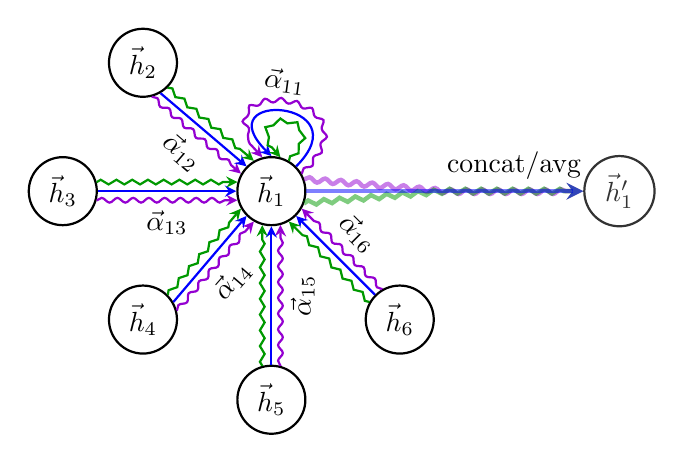
\begin{tikzpicture}

	\node[circle, draw, thick] (h1) {$\vec{h}_1$};
	\node[circle, draw, thick, above left=of h1] (h4) {$\vec{h}_2$};
	\node[circle, draw, thick, left=5em of h1] (h5) {$\vec{h}_3$};
	\node[circle, draw, thick, below left=of h1] (h6) {$\vec{h}_4$};
	\node[circle, draw, thick, below=5em of h1] (h7) {$\vec{h}_5$};
	\node[circle, draw, thick, below right=of h1] (h8) {$\vec{h}_6$};
	
	\draw[-stealth, mymauve, thick,decoration={snake, pre length=0.01mm, segment length=2mm, amplitude=0.3mm, post length=1.5mm}, decorate] (h8.120) -- node[sloped, above, black] {$\vec{\alpha}_{16}$} (h1.-30);
	\draw[-stealth, blue, thick] (h8.135) -- (h1.-45);
	\draw[-stealth, mygreen, thick, decoration={zigzag, pre length=0.01mm, segment length=2mm, amplitude=0.3mm, post length=1.5mm}, decorate] (h8.150) -- (h1.-60);
	
	\draw[-stealth, mymauve, thick,decoration={snake, pre length=0.01mm, segment length=2mm, amplitude=0.3mm, post length=1.5mm}, decorate] (h1.30) to[looseness=7] node[sloped, above, black] {$\vec{\alpha}_{11}$}(h1.105);
	\draw[-stealth, blue, thick] (h1.45) to[looseness=9] (h1.90);
	\draw[-stealth, mygreen, thick, decoration={zigzag, pre length=0.01mm, segment length=2mm, amplitude=0.3mm, post length=1.5mm}, decorate] (h1.60) to[looseness=20] (h1.75);
	
	\draw[-stealth, mymauve, thick,decoration={snake, pre length=0.01mm, segment length=2mm, amplitude=0.3mm, post length=1.5mm}, decorate] (h4.285) -- node[sloped, below, black] {$\vec{\alpha}_{12}$}(h1.150);
	\draw[-stealth, blue, thick] (h4.300) -- (h1.135);
	\draw[-stealth, mygreen, thick, decoration={zigzag, pre length=0.01mm, segment length=2mm, amplitude=0.3mm, post length=1.5mm}, decorate] (h4.315) -- (h1.120);
	
	\draw[-stealth, mymauve, thick,decoration={snake, pre length=0.01mm, segment length=2mm, amplitude=0.3mm, post length=1.5mm}, decorate] (h5.-15) -- node[sloped, below, black] {$\vec{\alpha}_{13}$}(h1.195);
	\draw[-stealth, blue, thick] (h5.0) -- (h1.180);
	\draw[-stealth, mygreen, thick, decoration={zigzag, pre length=0.01mm, segment length=2mm, amplitude=0.3mm, post length=1.5mm}, decorate] (h5.15) -- (h1.165);
	
		\draw[-stealth, mymauve, thick,decoration={snake, pre length=0.01mm, segment length=2mm, amplitude=0.3mm, post length=1.5mm}, decorate] (h6.15) -- node[sloped, below, black] {$\vec{\alpha}_{14}$}(h1.240);
	\draw[-stealth, blue, thick] (h6.30) -- (h1.225);
	\draw[-stealth, mygreen, thick, decoration={zigzag, pre length=0.01mm, segment length=2mm, amplitude=0.3mm, post length=1.5mm}, decorate] (h6.45) -- (h1.210);
	
	\draw[-stealth, mymauve, thick,decoration={snake, pre length=0.01mm, segment length=2mm, amplitude=0.3mm, post length=1.5mm}, decorate] (h7.75) -- node[sloped, below, black] {$\vec{\alpha}_{15}$}(h1.-75);
	\draw[-stealth, blue, thick] (h7.90) -- (h1.-90);
	\draw[-stealth, mygreen, thick, decoration={zigzag, pre length=0.01mm, segment length=2mm, amplitude=0.3mm, post length=1.5mm}, decorate] (h7.105) -- (h1.-105);
	
	\node[circle, draw, thick, right=10em of h1, opacity=0.8] (hp) {$\vec{h}_1'$};
	
	\coordinate[right=5em of h1] (A);
	
	\draw[-stealth,  mymauve, opacity=0.5, ultra thick,decoration={snake, pre length=0.01mm, segment length=2mm, amplitude=0.3mm, post length=1.5mm}, decorate] (h1.20) -- (A) -- (hp);
	\draw[-stealth, mygreen, opacity=0.5, ultra thick,decoration={zigzag, pre length=0.01mm, segment length=2mm, amplitude=0.3mm, post length=1.5mm}, decorate] (h1.-20) -- (A) -- (hp);
	\draw[-stealth, blue, opacity=0.5, ultra thick] (h1.0) -- (A) -- node[black, above, opacity=1.0] {concat/avg} (hp);

\end{tikzpicture}




\end{figure}

Furthermore, the directed multigraph setting we described in section
\ref{sec:catboost_model} is not a problem for the GAT model, since it
can handle multiple edges between the same pair of nodes, as we will
show in the following sections. We show how we model the GAT to be a
directed multigraph representing the flights and their features in
Figure \ref{fig:multigraph_layer}.


\begin{figure}[h]
  \centering
  \begin{tikzpicture}
    % Define colors for different attention heads
    \definecolor{color1}{RGB}{60, 120, 216}  % Blue
    \definecolor{color2}{RGB}{34, 139, 34}   % Green
    \definecolor{color3}{RGB}{255, 99, 71}   % Red

    % Define nodes
    \node[circle, draw, thick] (node1) at (0,0) {$\vec{h}_{\text{SP}}$};
    \node[circle, draw, thick] (node2) at (5,0) {$\vec{h}_{\text{RJ}}$};

    % Flight 1: alternating colors for attention heads
    \draw[-stealth, thick, color1!150] (node1) .. controls +(1,2) and +(-1,2) .. node[midway, above, black] {$\vec{\alpha}_{\text{SP},\text{RJ}}^{(\text{\faPlane}_1)}$} (node2);
    \draw[-stealth, thick, color2!150, dashed] (node1) .. controls +(1,1.5) and +(-1,1.5) .. node[midway, above, color2] {} (node2);
    \draw[-stealth, thick, color3!150, dotted] (node1) .. controls +(1,1) and +(-1,1) .. node[midway, above, color3] {} (node2);

    % Flight 2: same color pattern but lighter shades
    \draw[-stealth, thick, color1!100] (node1) .. controls +(1,-1) and +(-1,-1) .. node[midway, below, color1!70] {} (node2);
    \draw[-stealth, thick, color2!100, dashed] (node1) .. controls +(1,-1.5) and +(-1,-1.5) .. node[midway, below, black] {$\vec{\alpha}_{\text{SP},\text{RJ}}^{(\text{\faPlane}_2)}$} (node2);
    \draw[-stealth, thick, color3!100, dotted] (node1) .. controls +(1,-2) and +(-1,-2) .. node[midway, below, color3!70] { } (node2);

    % Flight 3: same color pattern but even lighter shades
    \draw[-stealth, thick, color1!50] (node1) .. controls +(1,-3) and +(-1,-3) .. node[midway, below, color1!50] { } (node2);
    \draw[-stealth, thick, color2!50, dashed] (node1) .. controls +(1,-3.5) and +(-1,-3.5) .. node[midway, below, color2!50] { } (node2);
    \draw[-stealth, thick, color3!50, dotted] (node1) .. controls +(1,-4) and +(-1,-4) .. node[midway, below, black] {$\vec{\alpha}_{\text{SP},\text{RJ}}^{(\text{\faPlane}_3)}$} (node2);

    % Output node
    \node[circle, draw, thick, right=7em of node2, opacity=0.8] (output) {$\vec{h}_{\text{RJ}}'$};

    % Aggregation line with label
    % \draw[-stealth, thick, color1!70] (node2) -- ++(1.5,0) -- ++(1.5,0) node[midway, above, black] {concat/avg} -- (output);

    \draw[-stealth,  color1, opacity=0.5, ultra thick,decoration={snake, pre length=0.01mm, segment length=2mm, amplitude=0.3mm, post length=1.5mm}, decorate] (node2.20)  -- (output);
    \draw[-stealth, color3, opacity=0.5, ultra thick,decoration={zigzag, pre length=0.01mm, segment length=2mm, amplitude=0.3mm, post length=1.5mm}, decorate] (node2.-20)  -- (output);
    \draw[-stealth, color2, opacity=0.5, ultra thick] (node2.0)  -- node[black, above, opacity=1.0] {concat/avg} (output);

  \end{tikzpicture}
  \caption{Airport multigraph GAT Layer with multi-head attention for three different flights between nodes (SP,RJ), with alternating colors opacity for each flight.}
  \label{fig:multigraph_layer}
\end{figure}


Finally, the last layer of our predictor would be to pass the learned
node embeddings $h_i$ and $h_j$ with the edge feature $e_{ij}^{(k)}$
of the flight $k$ to a fully connected layer (MLP) to predict the
holding of the flight $k$.  That is, we simply concatenate them, and
after the MLP layer, we have a sigmoid $\sigma$ activation function that
outputs the prediction $\hat{y}_k$ of holding,

$$ \hat{y}_k = \sigma (\text{MLP}(h_i || h_j || e_{ij}^{(k)})) \; \; \; \text{.} $$


\chapter{Results}
\label{Results}

% In this chapter, we describe the experiments conducted, beginning with the experimental setup and technology settings used (Section \ref{sec:setup}). We then compare the heuristic with the exact model using a fixed $T$ (obtained by the heuristic) (Section \ref{sec:comparison}), and finally, we present the phase transition in the heuristic, normalizing by individual drone paths (Section \ref{sec:transition}). This approach allows us to illustrate the advantages and limitations of our method.

% All experiments were performed on a 64-bit operating system with an Intel(R) Core(TM) i7-7700 CPU @ 3.60GHz and 16GB of RAM.

% \section{Experimental Setup and Technologies}
% \label{sec:setup}

% All experiments were conducted using the following software and tools:

% \subsection{Heuristic Implementation in C\texttt{++}}

% The heuristic approach was implemented in C\texttt{++}, chosen for its efficiency and control over system resources. Key components include:

% \begin{itemize}
% \item \textbf{Standard Library Containers}: The heuristic utilized standard C\texttt{++} library containers such as \texttt{vector} and \texttt{map} for efficient data management and manipulation. 
% \item \textbf{Version and Compiler}: The implementation made use of C\texttt{++}20, and the code was compiled using the GNU GCC compiler.
% \end{itemize}

% \subsection{Exact Model Implementation in Julia}

% The exact model was implemented in Julia, chosen for its high-performance capabilities and ease of use in mathematical and scientific computing. Key aspects include:

% \begin{itemize}
% \item \textbf{JuMP Package}: The exact model's optimization tasks were carried out using the \texttt{JuMP} package \cite{JuMPLubin2023}, a domain-specific modeling language for mathematical optimization embedded in Julia.
% \item \textbf{Gurobi Solver}: Gurobi was used as the Mixed-Integer Linear Programming (MILP) solver, interfaced through Julia, to solve the optimization problems with high precision and performance.
% \end{itemize}

% \subsection{Experimentation and Analysis}

% The comparison, experiments, and plots were conducted in Julia. The workflow included the following steps:

% \begin{itemize}
% \item \textbf{Calling C\texttt{++} Heuristic}: The compiled C\texttt{++} heuristic code was called externally from Julia. Input data was passed as files to the C\texttt{++} program.
% \item \textbf{Data Handling}: The output from the C\texttt{++} heuristic was read back into Julia for further analysis.
% \item \textbf{Visualization}: Results were plotted using the \texttt{Plots.jl} package in Julia.
% \end{itemize}

% \subsection{Drone Generation}

% The experimental setup involved generating random samples for the drones' initial and final positions, varying the number of drones and the size of the grid. For each drone $k \in \{1, \ldots, K\}$, where $K$ is the current number of drones, the starting position $(x_k^{\text{start}}, y_k^{\text{start}})$ and ending position $(x_k^{\text{end}}, y_k^{\text{end}})$ were randomly selected within a grid of size $N \times M$, where $N$ and $M$ are the dimensions of the grid.

% Formally, for each number of drones $K \in \{1, \ldots, R\}$, where $R$ is the maximum number of drones, and for each sample/trial $s \in \{1, \ldots, S\}$, the following procedure was applied:

% \begin{itemize}
% \item \textbf{Drone Generation}: For each drone $k \in \{1, \ldots, K\}$:
%   \begin{itemize}
%   \item Randomly generate $(x_k^{\text{start}}, y_k^{\text{start}}) \in \{1, \ldots, N\} \times \{1, \ldots, M\}$
%   \item Randomly generate $(x_k^{\text{end}}, y_k^{\text{end}}) \in \{1, \ldots, N\} \times \{1, \ldots, M\}$, ensuring $(x_k^{\text{end}}, y_k^{\text{end}}) \neq (x_k^{\text{start}}, y_k^{\text{start}})$
%   \end{itemize}
% \end{itemize}

% \section{Models Comparison}
% \label{sec:comparison}

% In this section, we compare the two models in terms of optimality(objective performance) and computational efficiency(running time). The x-axis in each plot represents the number of drones used to generate 20 samples per number of drones in the box plots, conducted in a 5x5 grid. The input $T$ for the exact model in each sample is the one returned by the heuristic, that is, $ T_{\text{exact\_model}} \vcentcolon  = T_{\text{heuristic}}$.

% \subsection{Objective Function Performance}

% We first evaluate the performance of both models in terms of their objective function outcomes. The objective function (y-axis) represents the optimization goal of minimizing path lengths for drones while avoiding collisions. Figure \ref{fig:exact_model_obj} and Figure \ref{fig:heuristic_obj} depict box plots comparing the objective function values achieved by the exact model and the heuristic model, respectively. 

% Figure \ref{fig:exact_model_obj} presents the distribution of objective function values obtained by the exact model, illustrating the spread and central tendency of the outcomes across different scenarios. Conversely, Figure \ref{fig:heuristic_obj} showcases the corresponding results for the heuristic model. By comparing these plots, we can gain valuable insights into the performance of each model in optimizing the objective function.

% In the scenario where $n_{\text{drones}} = 1$, the heuristic model performs as optimally as the exact model since the BFS guarantees optimality in this simple case. However, as the number of drones increases, the performance of the heuristic model diminishes. This decline in performance is anticipated due to the increased traffic within a fixed grid size, leading to more complex interactions and potential conflicts between the drones.


% \begin{figure}[H]
%     \centering
%     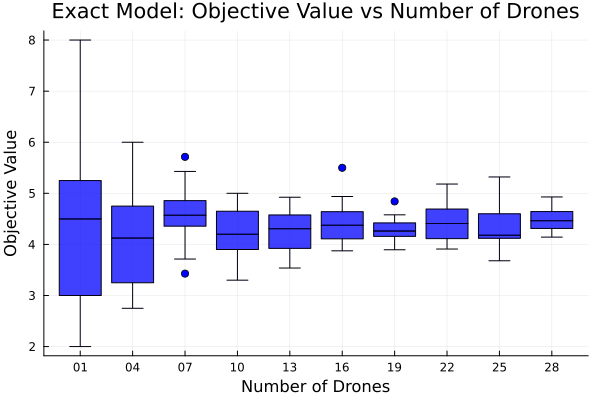
\includegraphics[width=0.8\textwidth]{img/julia_obj_boxplot_vs_drones.png}
%     \caption{Exact Model Objective. Source: The authors.}
%     \label{fig:exact_model_obj}
% \end{figure}

% \begin{figure}[H]
%     \centering
%     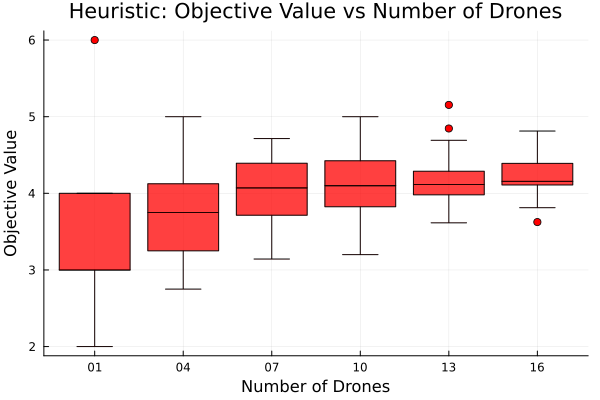
\includegraphics[width=0.8\textwidth]{img/cpp_obj_boxplot_vs_drones.png}
%     \caption{Heuristic Objective. Source: The authors.}
%     \label{fig:heuristic_obj}
% \end{figure}


% \subsection{Computational Efficiency}

% Next, we analyze the computational efficiency of the two models, focusing on the time required (y-axis) to compute the optimal paths for drones. Figures \ref{fig:exact_model_time} and \ref{fig:heuristic_time} display box plots representing the computational time taken by the exact model and the heuristic model, respectively. 

% Figure \ref{fig:exact_model_time} illustrates the distribution of computational times for the exact model. This plot provides an understanding of the computational overhead associated with solving the optimization problem precisely. Conversely, Figure \ref{fig:heuristic_time} presents the computational times required by the heuristic model. By comparing these plots, we assess the trade-off between computational efficiency and solution optimality offered by each model.

% As illustrated in Figure \ref{fig:exact_model_time}, the heuristic consistently exhibits a lower running time compared to the exact model. This disparity in running times is not merely a constant difference but reflects the inherent differences in computational complexity between the two approaches. The heuristic model demonstrates an almost constant running time, attributed to its sub-linear performance relative to the number of drones, as discussed in Section \ref{secc:complexity_analysis}. In contrast, the exact model, being NP-complete, has constraints that cause its performance to depend exponentially on both the number of drones and the specified $T$. Consequently, the running time of the exact model increases exponentially with the number of drones, as evidenced by the plot in Figure \ref{fig:exact_model_time}.


% \begin{figure}[H]
%     \centering
%     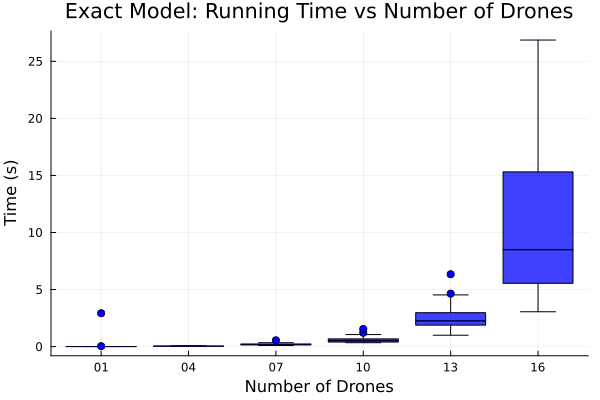
\includegraphics[width=0.8\textwidth]{img/julia_time_boxplot_vs_drones.png}
%     \caption{Exact Model time. Source: The authors.}
%     \label{fig:exact_model_time}
% \end{figure}

% \begin{figure}[H]
%     \centering
%     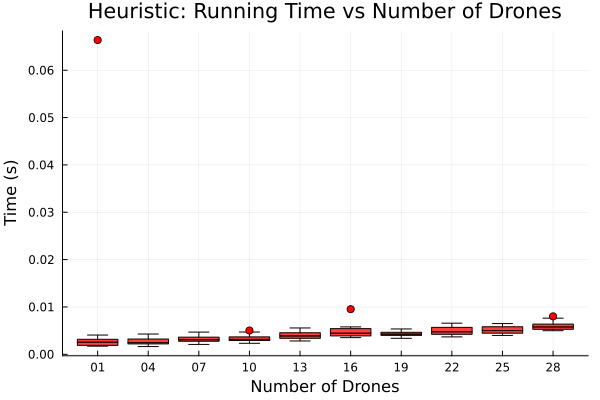
\includegraphics[width=0.8\textwidth]{img/cpp_time_boxplot_vs_drones.png}
%     \caption{Heuristic time. Source: The authors.}
%     \label{fig:heuristic_time}
% \end{figure}

% \subsection{Heuristic Behavior and Transition}
% \label{sec:transition}

% In this section, we propose an experimental setup to analyze the behavior of the heuristic in high-traffic configurations. We compare the heuristic's performance with the optimal distance for each drone in a collision-free environment, where the optimal path for each drone does not consider other drones in the grid (Manhattan distance).

% Primarily, we define the optimal distance per drone as the Manhattan distance between its start and end points. For each drone $k \in \mathcal{R}$, with starting position $(x_k^{\text{start}}, y_k^{\text{start}})$ and ending position $(x_k^{\text{end}}, y_k^{\text{end}})$, the Manhattan distance $D_k$ is given by: \[
% D_k = |x_k^{\text{start}} - x_k^{\text{end}}| + |y_k^{\text{start}} - y_k^{\text{end}}|\text{.}
% \]

% We then calculate the actual path length $P_k$ for each drone $k$ based on the heuristic path, and compute the optimality ratio $R_k$ as follows: \[
% R_k = \frac{P_k}{D_k}\text{.}
% \]

% The optimality ratio provides a measure of how efficiently the heuristic performs compared to the ideal (collision-free) path.

% The experiments were conducted using a $6 \times 6$ grid with the number of drones ranging from 1 to 99. For each number of drones, 30 points were sampled.

% The visualization of the heuristic performance can be measured in several ways. For our purpose, we chose two metrics:

% \begin{itemize}
%     \item \textbf{Normalized Distance}: This metric shows the actual path length taken by each drone normalized by the Manhattan distance. It illustrates how the heuristic manages to find paths in high-traffic scenarios compared to the optimal path lengths.
% \end{itemize}

% \begin{figure}[H]
%     \centering
%     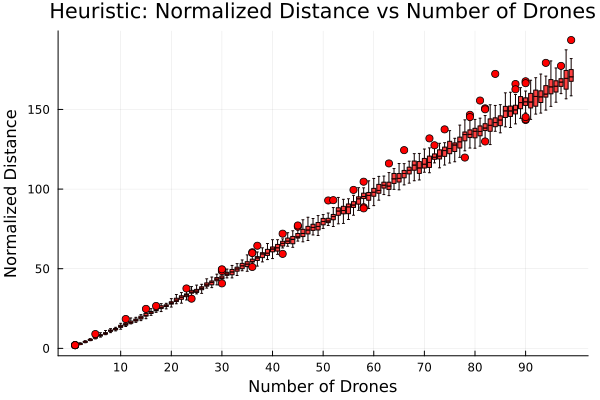
\includegraphics[width=0.8\textwidth]{img/cpp_normalized_distance_boxplot_vs_drones.png}
%     \caption{Heuristic normalized distance per drone. Source: The authors.}
%     \label{fig:heuristic_normalized_dist}
% \end{figure}

% Figure \ref{fig:heuristic_normalized_dist} displays the distribution of normalized distances for the heuristic, highlighting how the path lengths vary with an increasing number of drones. The box plot provides insights into the spread and central tendency of the heuristic's performance.

% \begin{itemize}
%     \item \textbf{Routing Time ($T$)}: This metric shows the time taken for the heuristic to compute the paths for all drones. It provides an understanding of the computational efficiency of the heuristic as the traffic increases.
% \end{itemize}

% \begin{figure}[H]
%     \centering
%     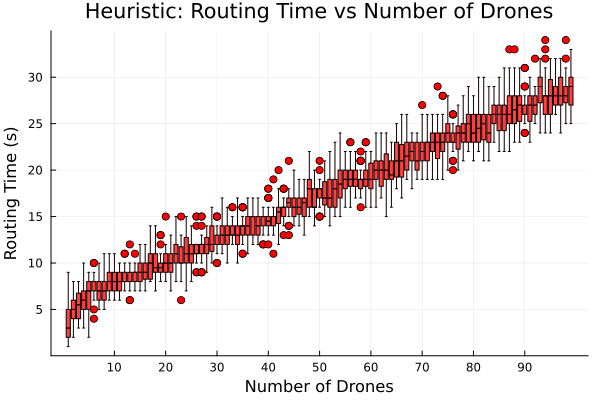
\includegraphics[width=0.8\textwidth]{img/cpp_routing_time_boxplot_vs_drones.png}
%     \caption{Heuristic Routing Time ($T$) corresponding to Figure \ref{fig:heuristic_normalized_dist}. Source: The authors.}
%     \label{fig:heuristic_normalized_routing_time}
% \end{figure}

% Figure \ref{fig:heuristic_normalized_routing_time} illustrates the routing times required by the heuristic as the number of drones increases. The box plot shows the variability in routing times and helps identify any trends or outliers. This result evinces the reasonability of the hybrid method in \ref{Hybrid_Methodology}, since we have a T that increases just linearly in the number of drones, even in a high traffic condition(36 cells available cells and 99 drones).

% Together, these figures provide a comprehensive view of the heuristic's behavior under varying traffic conditions, demonstrating both its effectiveness in finding feasible paths and its computational efficiency. 

% -----------------------------------------------------------
% Referências bibliográficas
% ----------------------------------------------------------

\newpage

%---------------------------------------------------------------------

\bibliographystyle{plainnat}
\bibliography{8_references}

\end{document}
